\documentclass[sumario=abnt-6027-2012]{ifes8}

\usepackage[utf8]{inputenc}
\usepackage{graphicx}
\usepackage{float}
\usepackage{caption}
\usepackage{subcaption}
\usepackage{array}
\usepackage{booktabs}
\usepackage{url}
\usepackage{amssymb}
\usepackage{amsmath}

% -----------------------------------------------------------------
% Identificação
% -----------------------------------------------------------------
\titulo{Laboratório 01: Linguagens Regulares}
\autor{Flávio Miozzi Batista}
\local{Serra}
\data{2026}
\orientador{Prof. Jefferson Oliveira Andrade}
\instituicao{Instituto Federal do Espírito Santo}
\curso{Mestrado Profissional em Computação Aplicada}
\preambulo{Relatório de atividade de laboratório apresentado ao
  Mestrado Profissional em Computação Aplicada do Instituto Federal do
  Espírito Santo como parte das atividades da disciplina Teoria da
  Computação, semestre 2026/1.}

% -----------------------------------------------------------------
% Comandos auxiliares
% -----------------------------------------------------------------
\newcommand{\rx}[1]{\texttt{#1}}           % expressão regular em monoespaço
\newcommand{\celula}[1]{\textbf{#1}}       % célula da grade
\newcommand{\heart}{\ensuremath{\heartsuit}} % símbolo especial nos puzzles

% -----------------------------------------------------------------
\begin{document}

\imprimircapa

\begin{folhaderosto}
\end{folhaderosto}

\pdfbookmark[0]{\contentsname}{toc}
\tableofcontents*
\cleardoublepage

\textual

% =================================================================
\chapter{Atividade Complementar: Regex Crossword}
% =================================================================

\section{Introdução}

\textit{Regex Crossword} é uma plataforma de quebra-cabeças interativos
disponível em \url{https://regexcrossword.com}, na qual o objetivo é
preencher uma grade bidimensional com caracteres de modo que cada linha
e cada coluna satisfaça simultaneamente a expressão regular especificada
como restrição. A atividade exercita, de maneira lúdica, a capacidade
do aluno de construir e interpretar expressões regulares — habilidade
central na disciplina de Teoria da Computação.

Este capítulo apresenta as soluções para os cinco desafios da seção
\textit{Beginner} e, em seguida, descreve dois quebra-cabeças originais
criados e publicados pelo aluno na seção \textit{Player Puzzles}.

% -----------------------------------------------------------------
\section{Desafios da Seção \textit{Beginner}}
% -----------------------------------------------------------------

A seção \textit{Beginner} compreende cinco desafios introdutórios, cada
um com grade 2×2. A Figura~\ref{fig:desafios-concluidos} apresenta a
visão geral dos cinco desafios concluídos com indicação de resolução
completa.

\begin{figure}[H]
  \centering
  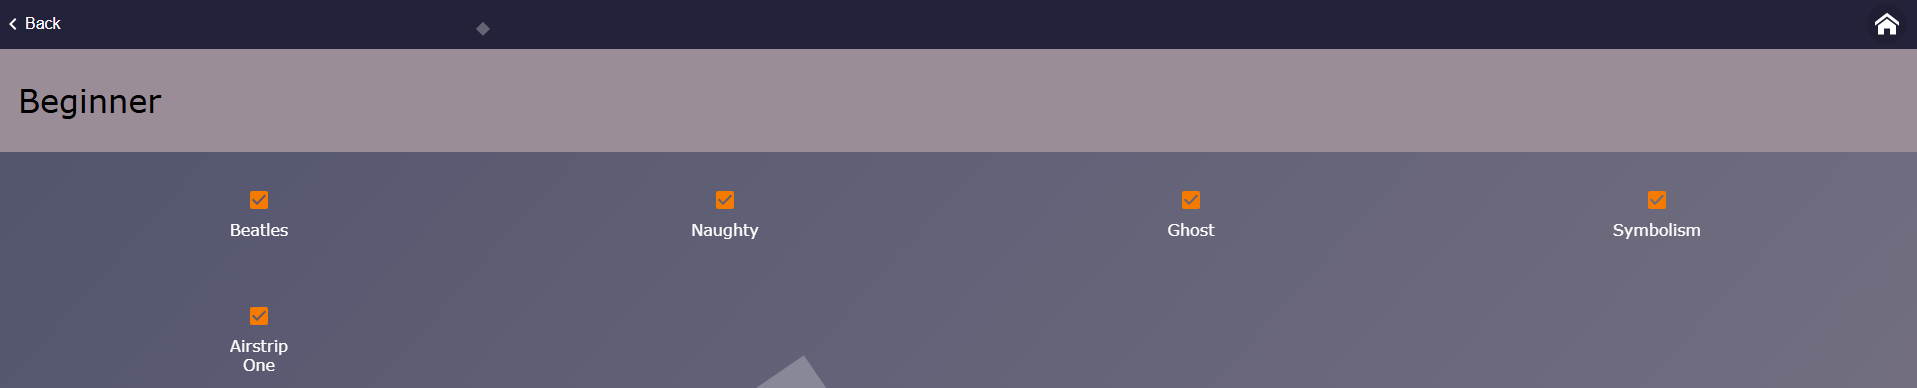
\includegraphics[width=0.9\textwidth]{img/regexcrossword_Desafios_Concluidos.png}
  \caption{Visão geral dos cinco desafios da seção \textit{Beginner}
    concluídos: Beatles, Naughty, Ghost, Symbolism e Airstrip One.}
  \label{fig:desafios-concluidos}
\end{figure}

% . . . . . . . . . . . . . . . . . . . . . . . . . . . . . . . .
\subsection{Desafio 1 — \textit{Beatles}}

O desafio \textit{Beatles} apresenta uma grade 2×2 com restrições que
combinam alternância e classes de caracteres. A solução é formada pelas
letras \celula{H}, \celula{E}, \celula{L}, \celula{P} — compondo a
palavra \textit{HELP}, título do álbum homônimo dos Beatles (1965).

\begin{figure}[H]
  \centering
  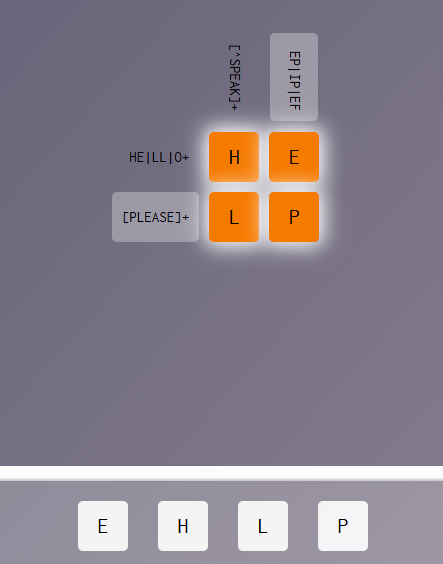
\includegraphics[width=0.38\textwidth]{img/Desafio_1.png}
  \caption{Desafio \textit{Beatles} — solução: HELP.}
  \label{fig:desafio1}
\end{figure}

\begin{center}
\begin{tabular}{c|c|c|}
  \multicolumn{1}{c}{} &
  \multicolumn{1}{c}{\rx{HE|LL|O+}} &
  \multicolumn{1}{c}{\rx{[PLEASE]+}} \\
  \cline{2-3}
  \rx{[*SPEAK]+} & \celula{H} & \celula{E} \\
  \cline{2-3}
  \rx{EP|IP|EF}  & \celula{L} & \celula{P} \\
  \cline{2-3}
\end{tabular}
\end{center}

% . . . . . . . . . . . . . . . . . . . . . . . . . . . . . . . .
\subsection{Desafio 2 — \textit{Naughty}}

O desafio \textit{Naughty} introduz o operador de referência reversa
(\rx{\textbackslash 1}), que exige que uma subcadeia coincidir com o
primeiro grupo de captura. A solução é \celula{B}, \celula{O},
\celula{B}, \celula{E} — formando a palavra \textit{BOBE}.

\begin{figure}[H]
  \centering
  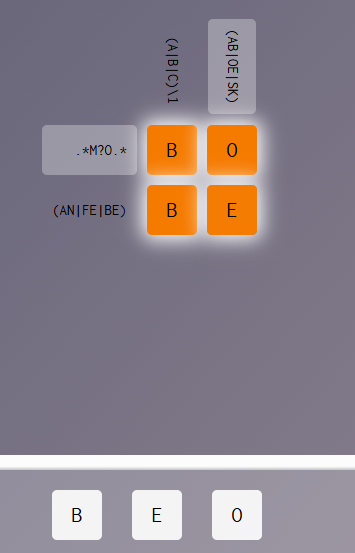
\includegraphics[width=0.38\textwidth]{img/Desafio_2.png}
  \caption{Desafio \textit{Naughty} — solução: BOBE.}
  \label{fig:desafio2}
\end{figure}

\begin{center}
\begin{tabular}{c|c|c|}
  \multicolumn{1}{c}{} &
  \multicolumn{1}{c}{\rx{(A|B|C)\textbackslash 1}} &
  \multicolumn{1}{c}{\rx{(AB|OE|SK)}} \\
  \cline{2-3}
  \rx{.*M?O.*}    & \celula{B} & \celula{O} \\
  \cline{2-3}
  \rx{(AN|FE|BE)} & \celula{B} & \celula{E} \\
  \cline{2-3}
\end{tabular}
\end{center}

Verificação:
\begin{itemize}
  \item Linha 1 (\textit{BO}): \rx{.*M?O.*} — \textit{B} casa \rx{.*},
    \textit{M?} é omitido, \textit{O} casa literalmente \checkmark
  \item Linha 2 (\textit{BE}): \rx{(AN|FE|BE)} — terceira alternativa \checkmark
  \item Coluna 1 (\textit{BB}): \rx{(A|B|C)\textbackslash 1} — grupo captura
    \textit{B}, referência \rx{\textbackslash 1} exige \textit{B} \checkmark
  \item Coluna 2 (\textit{OE}): \rx{(AB|OE|SK)} — segunda alternativa \checkmark
\end{itemize}

% . . . . . . . . . . . . . . . . . . . . . . . . . . . . . . . .
\subsection{Desafio 3 — \textit{Ghost}}

No desafio \textit{Ghost}, todas as quatro células recebem o caractere
\celula{O}, compondo a solução \textit{OOOO}.

\begin{figure}[H]
  \centering
  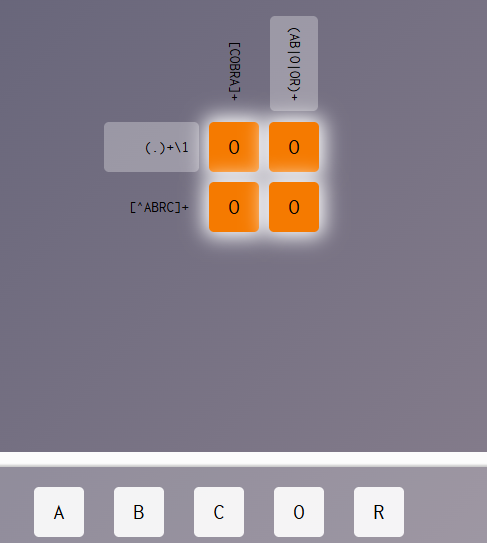
\includegraphics[width=0.38\textwidth]{img/Desafio_3.png}
  \caption{Desafio \textit{Ghost} — solução: OOOO.}
  \label{fig:desafio3}
\end{figure}

\begin{center}
\begin{tabular}{c|c|c|}
  \multicolumn{1}{c}{} &
  \multicolumn{1}{c}{\rx{[COBRA]+}} &
  \multicolumn{1}{c}{\rx{(AB|O|OR)+}} \\
  \cline{2-3}
  \rx{(.)+\textbackslash 1} & \celula{O} & \celula{O} \\
  \cline{2-3}
  \rx{[\textasciicircum ABRC]+} & \celula{O} & \celula{O} \\
  \cline{2-3}
\end{tabular}
\end{center}

Verificação:
\begin{itemize}
  \item Linha 1 (\textit{OO}): \rx{(.)+\textbackslash 1} — \rx{(.)} captura \textit{O},
    \rx{+} itera, \rx{\textbackslash 1} exige novo \textit{O} \checkmark
  \item Linha 2 (\textit{OO}): \rx{[\textasciicircum ABRC]+} — \textit{O}
    $\notin$ \{A,B,R,C\} \checkmark
  \item Coluna 1 (\textit{OO}): \rx{[COBRA]+} — \textit{O} $\in$
    \{C,O,B,R,A\} \checkmark
  \item Coluna 2 (\textit{OO}): \rx{(AB|O|OR)+} — alternativa \textit{O}
    aplicada duas vezes \checkmark
\end{itemize}

% . . . . . . . . . . . . . . . . . . . . . . . . . . . . . . . .
\subsection{Desafio 4 — \textit{Symbolism}}

O desafio \textit{Symbolism} utiliza exclusivamente caracteres simbólicos
do alfabeto \{\rx{*}, \rx{+}, \rx{,}, \rx{/}\}. A solução é
\celula{*}, \celula{*}, \celula{/}, \celula{/}.

\begin{figure}[H]
  \centering
  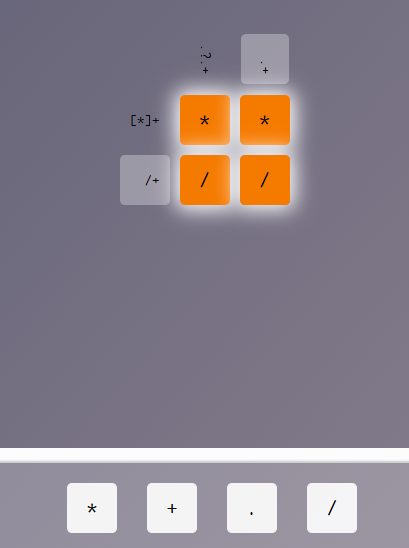
\includegraphics[width=0.38\textwidth]{img/Desafio_4.png}
  \caption{Desafio \textit{Symbolism} — solução: {*}{*}//.}
  \label{fig:desafio4}
\end{figure}

\begin{center}
\begin{tabular}{|c|c|}
\hline
\celula{*} & \celula{*} \\
\hline
\celula{/} & \celula{/} \\
\hline
\end{tabular}
\end{center}

O desafio explora o fato de que, dentro de classes de caracteres
(\rx{[\ldots]}), quantificadores como \rx{*} e \rx{+} perdem seu
significado especial e são tratados como literais. A restrição de linha 2
\rx{/+} exige um ou mais \rx{/} — a sequência \textit{//} satisfaz
diretamente \checkmark.

% . . . . . . . . . . . . . . . . . . . . . . . . . . . . . . . .
\subsection{Desafio 5 — \textit{Airstrip One}}

O desafio \textit{Airstrip One} utiliza dígitos do alfabeto
\{\rx{0}, \rx{1}, \rx{4}, \rx{6}, \rx{8}, \rx{9}\}. A solução é
\celula{1}, \celula{9}, \celula{8}, \celula{4} — formando o número
\textit{1984}, referência ao romance distópico de George Orwell (o título
\textit{Airstrip One} é o nome da Inglaterra no livro).

\begin{figure}[H]
  \centering
  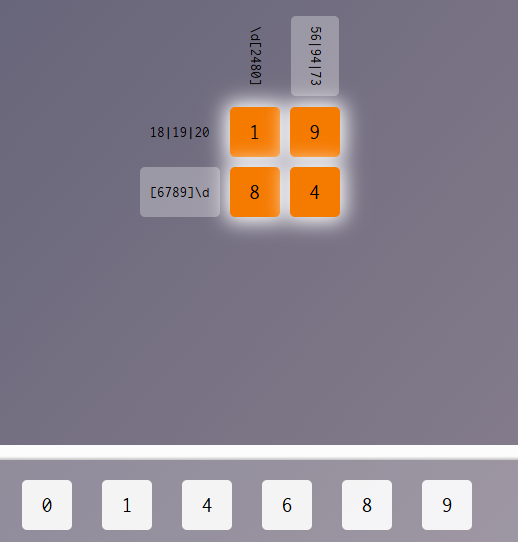
\includegraphics[width=0.38\textwidth]{img/Desafio_5.png}
  \caption{Desafio \textit{Airstrip One} — solução: 1984.}
  \label{fig:desafio5}
\end{figure}

\begin{center}
\begin{tabular}{c|c|c|}
  \multicolumn{1}{c}{} &
  \multicolumn{1}{c}{\rx{\textbackslash d[2480]}} &
  \multicolumn{1}{c}{\rx{56|94|73}} \\
  \cline{2-3}
  \rx{18|19|20}      & \celula{1} & \celula{9} \\
  \cline{2-3}
  \rx{[6789]\textbackslash d} & \celula{8} & \celula{4} \\
  \cline{2-3}
\end{tabular}
\end{center}

Verificação:
\begin{itemize}
  \item Linha 1 (\textit{19}): \rx{18|19|20} — segunda alternativa \checkmark
  \item Linha 2 (\textit{84}): \rx{[6789]\textbackslash d} — \textit{8}
    $\in$ \{6,7,8,9\}, \textit{4} $\in \Sigma_{dígitos}$ \checkmark
  \item Coluna 1 (\textit{18}): \rx{\textbackslash d[2480]} — \textit{1}
    $\in \Sigma_{dígitos}$, \textit{8} $\in$ \{2,4,8,0\} \checkmark
  \item Coluna 2 (\textit{94}): \rx{56|94|73} — segunda alternativa \checkmark
\end{itemize}

% -----------------------------------------------------------------
\section{Quebra-cabeças Criados pelo Aluno (\textit{Player Puzzles})}
% -----------------------------------------------------------------

Dois quebra-cabeças originais foram criados e publicados pelo aluno na
seção \textit{Player Puzzles} do \textit{Regex Crossword}. Ambos utilizam
referências ao nome do autor e à instituição de ensino.

% . . . . . . . . . . . . . . . . . . . . . . . . . . . . . . . .
\subsection{Quebra-cabeça 1 — FLAVIO\_HOUSE\_IFES (Grade 5×6)}

O quebra-cabeça \texttt{FLAVIO\_HOUSE\_IFES} é uma grade retangular de
5 linhas por 6 colunas, acessível em:
\begin{center}
  \url{https://regexcrossword.com/playerpuzzles/69ec93119f2fd}
\end{center}

As expressões regulares de linha foram projetadas para evocar palavras
associadas ao nome do autor, à família e à instituição. O alfabeto
utilizado inclui letras maiúsculas e o símbolo especial \heart{}.

\begin{figure}[H]
  \centering
  \begin{subfigure}[b]{0.47\textwidth}
    \centering
    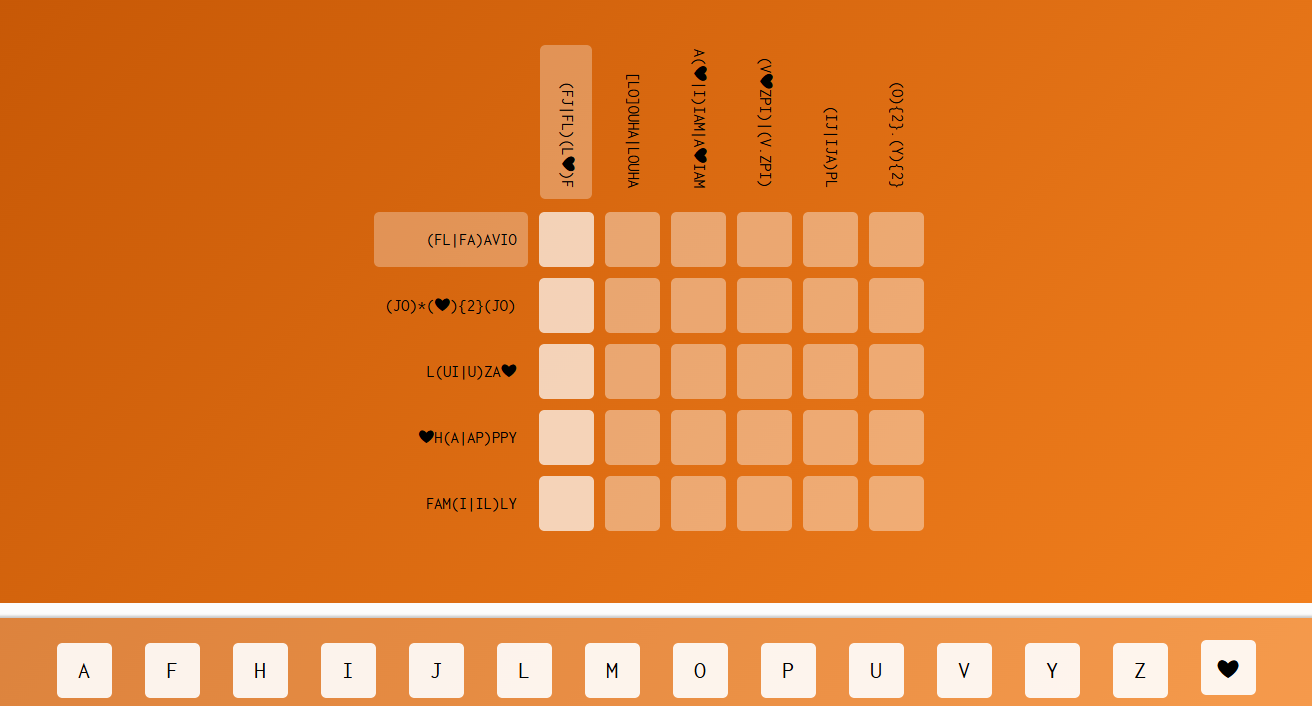
\includegraphics[width=\textwidth]{img/Player_Puzzles_FLAVIO_HOUSE_IFES_5X6.png}
    \caption{Quebra-cabeça sem solução.}
    \label{fig:puzzle1-unsolved}
  \end{subfigure}
  \hfill
  \begin{subfigure}[b]{0.47\textwidth}
    \centering
    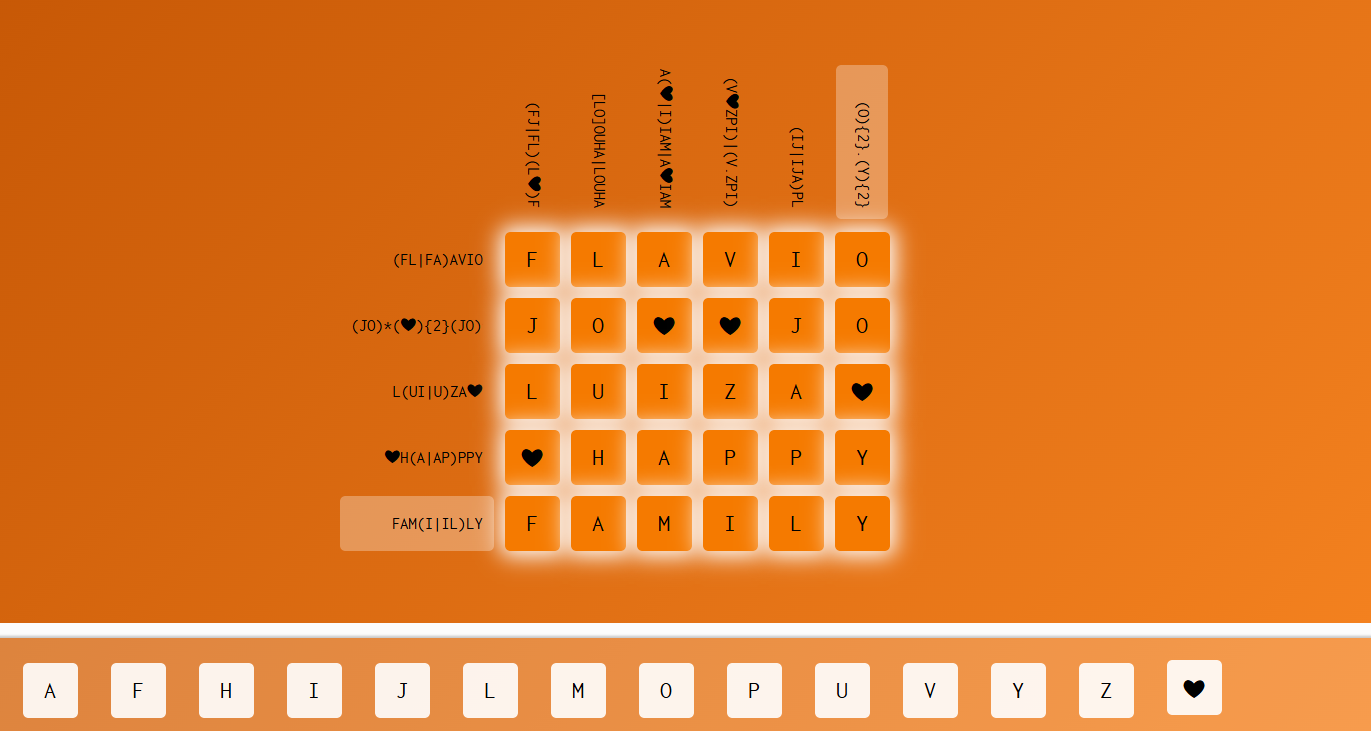
\includegraphics[width=\textwidth]{img/Player_Puzzles_FLAVIO_HOUSE_IFES_5X6_SOLVED.png}
    \caption{Quebra-cabeça com solução preenchida.}
    \label{fig:puzzle1-solved}
  \end{subfigure}
  \caption{Quebra-cabeça FLAVIO\_HOUSE\_IFES — grade retangular 5×6.}
  \label{fig:puzzle1}
\end{figure}

As restrições de linha projetadas são apresentadas na
Tabela~\ref{tab:puzzle1-linhas}.

\begin{table}[H]
  \centering
  \caption{Restrições de linha do quebra-cabeça FLAVIO\_HOUSE\_IFES.}
  \label{tab:puzzle1-linhas}
  \begin{tabular}{clp{6cm}}
    \toprule
    \textbf{Linha} & \textbf{Expressão Regular} & \textbf{Solução esperada} \\
    \midrule
    1 & \rx{(FL|FA)AVIO}        & FLAVIO \\
    2 & \rx{(JO)+\heart(2)(JO)} & JO\heart{}JO \\
    3 & \rx{L(UI|U)ZA\heart}    & LUZA\heart \\
    4 & \rx{\heart H(A|AP)PPY}  & \heart HAPPY \\
    5 & \rx{FAM(I|IL)Y}         & FAMILY \\
    \bottomrule
  \end{tabular}
\end{table}

% . . . . . . . . . . . . . . . . . . . . . . . . . . . . . . . .
\subsection{Quebra-cabeça 2 — FLAVIO\_MB\_IFES (Grade Hexagonal)}

O quebra-cabeça \texttt{FLAVIO\_MB\_IFES} é uma grade hexagonal de
tamanho 10 (arranjo 3-4-3), acessível em:
\begin{center}
  \url{https://regexcrossword.com/playerpuzzles/69ec8bdfb48b0}
\end{center}

A grade hexagonal impõe restrições em três direções — linhas horizontais
e duas diagonais — o que aumenta significativamente a complexidade do
design em comparação com grades retangulares. O alfabeto utilizado é
\{C, E, F, I, J, M, O, P, S\}.

\begin{figure}[H]
  \centering
  \begin{subfigure}[b]{0.47\textwidth}
    \centering
    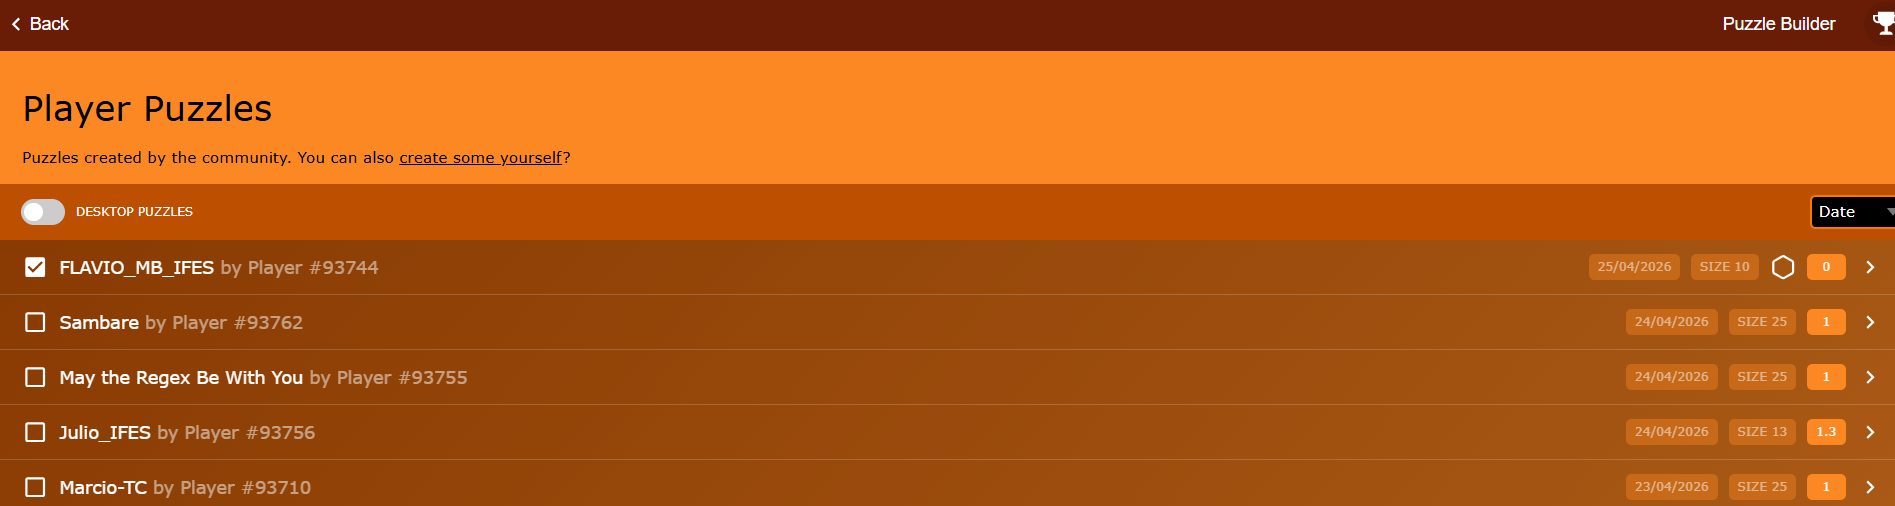
\includegraphics[width=\textwidth]{img/Player_Puzzles_FLAVIO_MB_IFES.png}
    \caption{Listagem do quebra-cabeça.}
    \label{fig:puzzle2-list}
  \end{subfigure}
  \hfill
  \begin{subfigure}[b]{0.47\textwidth}
    \centering
    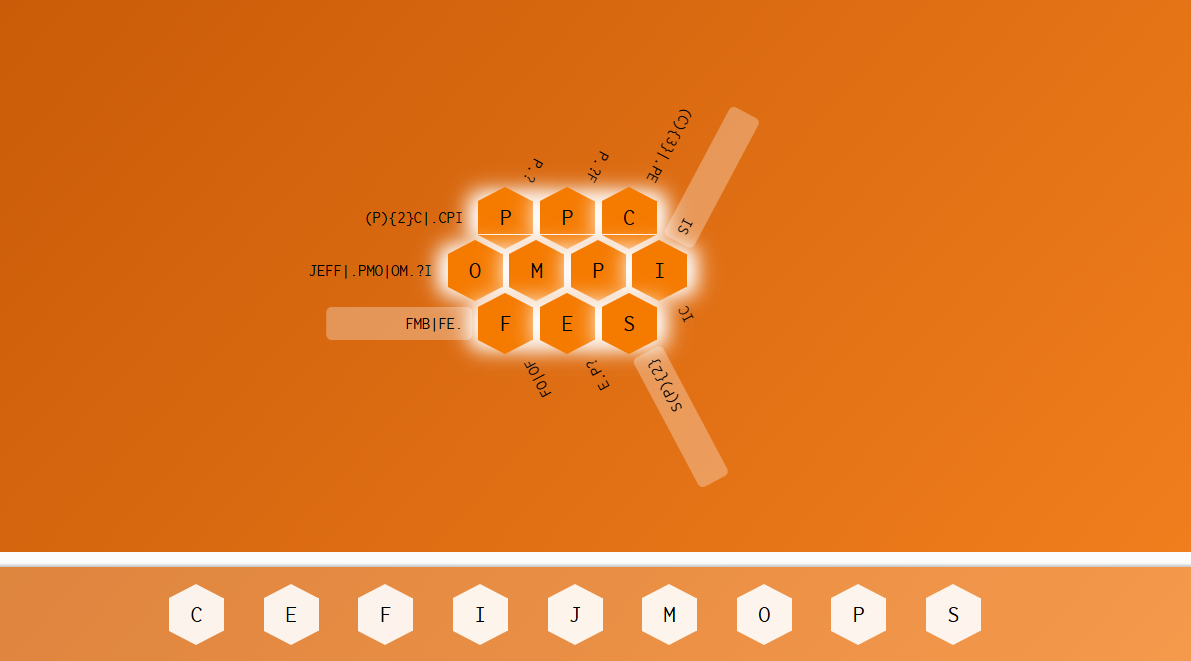
\includegraphics[width=\textwidth]{img/Player_Puzzles_FLAVIO_MB_IFES_Solved.png}
    \caption{Quebra-cabeça com solução preenchida.}
    \label{fig:puzzle2-solved}
  \end{subfigure}
  \caption{Quebra-cabeça FLAVIO\_MB\_IFES — grade hexagonal, tamanho 10.}
  \label{fig:puzzle2}
\end{figure}

A solução da grade hexagonal, lida linha a linha, compõe as letras:

\begin{center}
\begin{tabular}{ccc}
  \multicolumn{3}{c}{Linha 1: \celula{P} \celula{P} \celula{C}} \\
  \multicolumn{3}{c}{Linha 2: \celula{O} \celula{M} \celula{P} \celula{I}} \\
  \multicolumn{3}{c}{Linha 3: \celula{F} \celula{E} \celula{S}} \\
\end{tabular}
\end{center}

O resultado — \textit{PPC/OMPI/FES} — é uma referência ao
\textit{Programa de Pós-Graduação em Computação Aplicada} (PPCOMPI) do
Instituto Federal do Espírito Santo (IFES), programa ao qual o autor está
vinculado. As restrições de linha horizontais são apresentadas na
Tabela~\ref{tab:puzzle2-linhas}.

\begin{table}[H]
  \centering
  \caption{Restrições de linha do quebra-cabeça FLAVIO\_MB\_IFES.}
  \label{tab:puzzle2-linhas}
  \begin{tabular}{clp{5cm}}
    \toprule
    \textbf{Linha} & \textbf{Expressão Regular} & \textbf{Solução esperada} \\
    \midrule
    1 & \rx{(P)(2)C|CPI}   & PPC \\
    2 & \rx{JEFF|PMO|OM?I}  & OMPI \\
    3 & \rx{FMB|FE.}        & FES \\
    \bottomrule
  \end{tabular}
\end{table}

% =================================================================
\chapter{Parte 1 — Conversão de Autômatos Finitos}
% =================================================================

\section{Introdução}

\textit{Conteúdo a ser preenchido.}

% =================================================================
\chapter{Parte 2 — Expressões Regulares}
% =================================================================

\section{Introdução}

\textit{Conteúdo a ser preenchido.}

\end{document}
